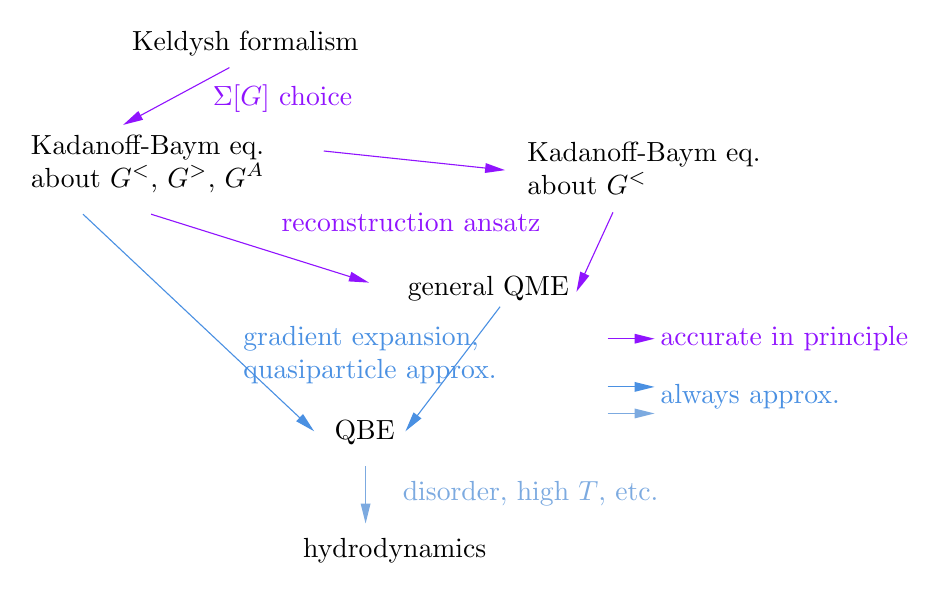
\begin{tikzpicture}[x=0.75pt,y=0.75pt,yscale=-0.8,xscale=0.8]
    %uncomment if require: \path (0,403); %set diagram left start at 0, and has height of 403
    
    %Straight Lines [id:da3574677469464902] 
    \draw [color={rgb, 255:red, 144; green, 19; blue, 254 }  ,draw opacity=1 ]   (226.17,66.27) -- (163.93,99.79) ;
    \draw [shift={(162.17,100.74)}, rotate = 331.69] [fill={rgb, 255:red, 144; green, 19; blue, 254 }  ,fill opacity=1 ][line width=0.08]  [draw opacity=0] (12,-3) -- (0,0) -- (12,3) -- cycle    ;
    %Straight Lines [id:da6278234902971178] 
    \draw [color={rgb, 255:red, 144; green, 19; blue, 254 }  ,draw opacity=1 ]   (179,154.55) -- (308.26,195.14) ;
    \draw [shift={(310.17,195.74)}, rotate = 197.43] [fill={rgb, 255:red, 144; green, 19; blue, 254 }  ,fill opacity=1 ][line width=0.08]  [draw opacity=0] (12,-3) -- (0,0) -- (12,3) -- cycle    ;
    %Straight Lines [id:da8214266493222495] 
    \draw [color={rgb, 255:red, 74; green, 144; blue, 226 }  ,draw opacity=1 ]   (138,154.55) -- (275.71,283.9) ;
    \draw [shift={(277.17,285.27)}, rotate = 223.21] [fill={rgb, 255:red, 74; green, 144; blue, 226 }  ,fill opacity=1 ][line width=0.08]  [draw opacity=0] (12,-3) -- (0,0) -- (12,3) -- cycle    ;
    %Straight Lines [id:da5242918677536943] 
    \draw [color={rgb, 255:red, 74; green, 144; blue, 226 }  ,draw opacity=1 ]   (389.17,210.27) -- (333.38,283.68) ;
    \draw [shift={(332.17,285.27)}, rotate = 307.23] [fill={rgb, 255:red, 74; green, 144; blue, 226 }  ,fill opacity=1 ][line width=0.08]  [draw opacity=0] (12,-3) -- (0,0) -- (12,3) -- cycle    ;
    %Straight Lines [id:da6748656000657882] 
    \draw [color={rgb, 255:red, 124; green, 170; blue, 224 }  ,draw opacity=1 ]   (308.17,306.27) -- (308.17,338.8) ;
    \draw [shift={(308.17,340.8)}, rotate = 270] [fill={rgb, 255:red, 124; green, 170; blue, 224 }  ,fill opacity=1 ][line width=0.08]  [draw opacity=0] (12,-3) -- (0,0) -- (12,3) -- cycle    ;
    %Straight Lines [id:da1182191617400088] 
    \draw [color={rgb, 255:red, 144; green, 19; blue, 254 }  ,draw opacity=1 ]   (283,116.49) -- (390.18,127.8) ;
    \draw [shift={(392.17,128.01)}, rotate = 186.02] [fill={rgb, 255:red, 144; green, 19; blue, 254 }  ,fill opacity=1 ][line width=0.08]  [draw opacity=0] (12,-3) -- (0,0) -- (12,3) -- cycle    ;
    %Straight Lines [id:da3233811707634906] 
    \draw [color={rgb, 255:red, 144; green, 19; blue, 254 }  ,draw opacity=1 ]   (457.17,153.41) -- (436,199.45) ;
    \draw [shift={(435.17,201.27)}, rotate = 294.68] [fill={rgb, 255:red, 144; green, 19; blue, 254 }  ,fill opacity=1 ][line width=0.08]  [draw opacity=0] (12,-3) -- (0,0) -- (12,3) -- cycle    ;
    %Straight Lines [id:da7080246790835758] 
    \draw [color={rgb, 255:red, 144; green, 19; blue, 254 }  ,draw opacity=1 ]   (454,229.55) -- (480.17,229.55) ;
    \draw [shift={(482.17,229.55)}, rotate = 180] [fill={rgb, 255:red, 144; green, 19; blue, 254 }  ,fill opacity=1 ][line width=0.08]  [draw opacity=0] (12,-3) -- (0,0) -- (12,3) -- cycle    ;
    %Straight Lines [id:da3562948391141818] 
    \draw [color={rgb, 255:red, 74; green, 144; blue, 226 }  ,draw opacity=1 ]   (454,258.55) -- (480.17,258.55) ;
    \draw [shift={(482.17,258.55)}, rotate = 180] [fill={rgb, 255:red, 74; green, 144; blue, 226 }  ,fill opacity=1 ][line width=0.08]  [draw opacity=0] (12,-3) -- (0,0) -- (12,3) -- cycle    ;
    %Straight Lines [id:da28735661944331214] 
    \draw [color={rgb, 255:red, 124; green, 170; blue, 224 }  ,draw opacity=1 ]   (454,274.55) -- (480.17,274.55) ;
    \draw [shift={(482.17,274.55)}, rotate = 180] [fill={rgb, 255:red, 124; green, 170; blue, 224 }  ,fill opacity=1 ][line width=0.08]  [draw opacity=0] (12,-3) -- (0,0) -- (12,3) -- cycle    ;
    
    % Text Node
    \draw (166,42.55) node [anchor=north west][inner sep=0.75pt]   [align=left] {Keldysh formalism};
    % Text Node
    \draw (258.1,84.99) node  [color={rgb, 255:red, 144; green, 19; blue, 254 }  ,opacity=1 ] [align=left] {$\displaystyle \Sigma [ G]$ choice};
    % Text Node
    \draw (105,105.55) node [anchor=north west][inner sep=0.75pt]   [align=left] {Kadanoff-Baym eq.\\about $\displaystyle G^{< }$, $\displaystyle G^{ >}$, $\displaystyle G^{\text{A}}$};
    % Text Node
    \draw (256,152.55) node [anchor=north west][inner sep=0.75pt]  [color={rgb, 255:red, 144; green, 19; blue, 254 }  ,opacity=1 ] [align=left] {reconstruction ansatz};
    % Text Node
    \draw (332,190.55) node [anchor=north west][inner sep=0.75pt]   [align=left] {general QME};
    % Text Node
    \draw (233,220.55) node [anchor=north west][inner sep=0.75pt]  [color={rgb, 255:red, 74; green, 144; blue, 226 }  ,opacity=1 ] [align=left] {gradient expansion,\\quasiparticle approx.};
    % Text Node
    \draw (288,277.55) node [anchor=north west][inner sep=0.75pt]   [align=left] {QBE};
    % Text Node
    \draw (329,314) node [anchor=north west][inner sep=0.75pt]  [color={rgb, 255:red, 124; green, 170; blue, 224 }  ,opacity=1 ] [align=left] {disorder, high $\displaystyle T$, etc.};
    % Text Node
    \draw (269,348) node [anchor=north west][inner sep=0.75pt]   [align=left] {hydrodynamics};
    % Text Node
    \draw (404,109.55) node [anchor=north west][inner sep=0.75pt]   [align=left] {Kadanoff-Baym eq.\\about $\displaystyle G^{< }$};
    % Text Node
    \draw (484.17,229.55) node [anchor=west] [inner sep=0.75pt]  [color={rgb, 255:red, 144; green, 19; blue, 254 }  ,opacity=1 ] [align=left] {accurate in principle};
    % Text Node
    \draw (484.17,264.55) node [anchor=west] [inner sep=0.75pt]  [color={rgb, 255:red, 74; green, 144; blue, 226}  ,opacity=1 ] [align=left] {always approx.};
    
    
    \end{tikzpicture}
    